\usetikzlibrary{positioning}
\usetikzlibrary{shapes}
\usetikzlibrary{fit}
\usetikzlibrary{backgrounds}
    
    
\section{CheatSheet}
\tikzstyle{mybox} = [draw=black, fill=white, 
    rectangle, inner sep=10pt, inner ysep=5pt]
% \tikzstyle{mybox} = [draw=black, fill=white, very thick,
%     rectangle, inner sep=10pt, inner ysep=5pt]
% \tikzstyle{mybox} = [draw=black, fill=white, very thick,
%     rectangle, rounded corners, inner sep=10pt, inner ysep=5pt]
\tikzstyle{fancytitle} =[fill=black, text=white, font=\bfseries]



\definecolor{DarkBackground}{HTML}{563D7C}
\definecolor{white}{HTML}{ffffff}

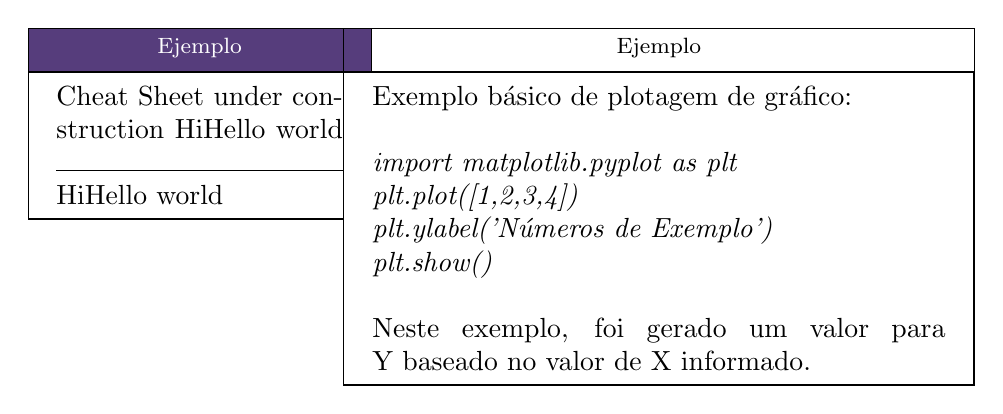
\begin{tikzpicture}
    % First box (1/3 of horizontal space)
    \node [mybox, minimum width=0.33\textwidth ,anchor=north west] at (0,0)(box1) {%
        \begin{minipage}{0.3\textwidth}
            Cheat Sheet under construction
            \LR{Hi}{Hello world} 
            \rule{\textwidth}{0.4pt}
            \LR{Hi}{Hello world} 
            % \LR{\lipsum[1]}{\lipsum[2]} 
            % \LR{\lipsum[1]}{\lipsum[2]} 

        \end{minipage}
    };
    % Second box (2/3 of horizontal space, aligned with the first box)
    \node [mybox, minimum width=0.66\textwidth, anchor=north west] at (0.33\textwidth,0)(box2) {%
    \begin{minipage}{0.6\textwidth}
        Exemplo básico de plotagem de gráfico:\\
        \\
        \textit{import matplotlib.pyplot as plt}\\
        \textit{plt.plot([1,2,3,4])}\\
        \textit{plt.ylabel('Números de Exemplo')}\\
        \textit{plt.show()}\\
        \\
        Neste exemplo, foi gerado um valor para Y baseado no valor de X informado.
    \end{minipage}
    };
    % Fancy titles for the boxes
        % Title node
    \node [above=0.05cm of box1, anchor=south,text=white] (title) {\footnotesize Ejemplo};
    \begin{scope}[on background layer]
        \node [draw, rectangle, fit=(box1)(title),inner sep=0pt,fill=DarkBackground] {};
    \end{scope}
    % \node[fancytitle, right=10pt] at (box1.north west) {Exemplo básico MatPlotLib:};
    \node [above=0.05cm of box2, anchor=south] (title2) {\footnotesize Ejemplo};
    \node [draw, rectangle, fit=(box2)(title2),inner sep=0pt] {};
    % \node[fancytitle, right=10pt] at (box2.north west) {Segundo Exemplo:};
\end{tikzpicture}



\section{Some numbers}
\subsection{Stirling numbers of the first kind}
    $stirlingI{n}{k}$ represents the number of permutations of $n$ elements in exactly $k$ disjoint cycles.
    \begin{align*}
        \stirlingI{0}{0} &= 1 \\
        \stirlingI{0}{n} &= \stirlingI{n}{0} = 0 \quad &, \quad n>0 \\
        \stirlingI{n}{k} &= (n-1)\stirlingI{n-1}{k} + \stirlingI{n-1}{k-1} \quad &, \quad k>0 \\
        \sum_{k=0}^{n} \stirlingI{n}{k} &= n! \\
        \sum_{k=0}^{\infty} \stirlingI{n}{k} x^k &= \prod_{k=0}^{n-1}(x+k)
    \end{align*}

\subsection{Stirling numbers of the second type}
    $stirlingII{n}{k}$ represents the number of ways to partition a set of $n$ distinguishable objects into $k$ nonempty subsets.
    \begin{align*}
        \stirlingII{0}{0} &= 1 \\
        \stirlingII{0}{n} &= \stirlingII{n}{0} = 0 \quad &, \quad n>0 \\
        \stirlingII{n}{k} &= k\stirlingII{n-1}{k} + \stirlingII{n-1}{k-1} \quad &, \quad k>0 \\
        &= \sum_{j=0}^{k} \dfrac{j^n}{j!} \cdot \dfrac{(-1)^{k-j}}{(k-j)!}
    \end{align*}

    \subsection{Euler numbers}
    $\euler{n}{k}$ represents the number of permutations from $1$ to $n$ where exactly $k$ numbers are greater than the previous number.
    \begin{align*}
        \euler{1}{0} &= 1 \\
        \euler{n}{k} &= (n-k)\euler{n-1}{k-1} + (k+1)\euler{n-1}{k} \quad &, \quad n \geq 2 \\
        &= \sum_{j=0}^{k} (-1)^j \binom{n+1}{j} (k+1-j)^n \\
        \sum_{k=0}^{n-1} \euler{n}{k} &= n!
    \end{align*}

\subsection{Catalan numbers}
    \begin{align*}
        C_0 &= 1 \\
        C_n &= \dfrac{1}{n+1}\binom{2n}{n} = \sum_{j=0}^{n-1} C_j C_{n-1-j} \\
        \sum_{n=0}^{\infty} C_n x^n &= \dfrac{1-\sqrt{1-4x}}{2x}
    \end{align*}
\begin{itemize}
    \item Parentheses Expressions: Catalan numbers count the number of different ways to arrange parentheses in a valid expression. For example, for n = 3, there are five valid expressions: ((())), ()(()), (())(), ()()(), and (()()).

    \item Binary Trees: They count the number of structurally different binary search trees with n nodes. Binary search trees are used in computer science for data storage and searching.

    \item Polygon Triangulations: In geometry, Catalan numbers count the ways to triangulate a convex polygon with n+2 sides, meaning the number of non-overlapping triangles formed by connecting n+2 vertices.


\end{itemize}

\subsection{Bell Numbers}
    $B_n$ represents the number of ways to partition a set of $n$ elements.
    \begin{align*}
        B_n &= \sum_{k=0}^{n}\stirlingII{n}{k} = \sum_{k=0}^{n-1}\binom{n-1}{k} B_k \\
        \sum_{n=0}^{\infty} \dfrac{B_n}{n!}x^n &= e^{e^x-1}
    \end{align*}

\subsection{Bernoulli numbers}
    \begin{align*}
        {B_0}^+ &= 1 \\
        {B_n}^+ &= 1 - \sum_{k=0}^{n-1}\binom{n}{k}\dfrac{{B_k}^+}{n-k+1} \\
        \sum_{n=0}^{\infty} \dfrac{{B_n}^+ x^n}{n!} &= \dfrac{x}{1-e^{-x}} = \dfrac{1}{\frac{1}{1!}-\frac{x}{2!}+\frac{x^2}{3!}-\frac{x^3}{4!}+\cdots}
    \end{align*}


    \section{Pythagorean Triples}
 The Pythagorean triples are uniquely generated by
 \[ a=k\cdot (m^{2}-n^{2}),\ \,b=k\cdot (2mn),\ \,c=k\cdot (m^{2}+n^{2}), \]
 with $m > n > 0$, $k > 0$, $m \bot n$, and either $m$ or $n$ even.

\section{Primes}
	$p=962592769$ is such that $2^{21} \mid p-1$, which may be useful. For hashing
	use 970592641 (31-bit number), 31443539979727 (45-bit), 3006703054056749
	(52-bit). There are 78498 primes less than 1\,000\,000.

	Primitive roots exist modulo any prime power $p^a$, except for $p = 2, a > 2$, and there are $\phi(\phi(p^a))$ many.
	For $p = 2, a > 2$, the group $\mathbb Z_{2^a}^\times$ is instead isomorphic to $\mathbb Z_2 \times \mathbb Z_{2^{a-2}}$.

\section{Estimates}
	$\sum_{d|n} d = O(n \log \log n)$.

	The number of divisors of $n$ is at most around 100 for $n < 5e4$, 500 for $n < 1e7$, 2000 for $n < 1e10$, 200\,000 for $n < 1e19$.

\section{Mobius Function}
\[
	\mu(n) = \begin{cases} 0 & n \textrm{ is not square free}\\ 1 & n \textrm{ has even number of prime factors}\\ -1 & n \textrm{ has odd number of prime factors}\\\end{cases}
\]
  Mobius Inversion:
  \[ g(n) = \sum_{d|n} f(d) \Leftrightarrow f(n) = \sum_{d|n} \mu(d)g(n/d) \]
  Other useful formulas/forms:

  $ \sum_{d | n} \mu(d) = [ n = 1] $ (very useful)

  $ g(n) = \sum_{n|d} f(d) \Leftrightarrow f(n) = \sum_{n|d} \mu(d/n)g(d)$

 $ g(n) = \sum_{1 \leq m \leq n} f(\left\lfloor\frac{n}{m}\right \rfloor ) \Leftrightarrow f(n) = \sum_{1\leq m\leq n} \mu(m)g(\left\lfloor\frac{n}{m}\right\rfloor)$


\section{Complexity}

- If problem is check for all multiples of a number in [1,n] and this multiples don´t exed maxn complexity is (maxn log(maxn))
- Sum of n/1+ n/2 + n/3 + n/4 + ... is nlogn
- Merge many sets can be do it in n logn if we insert elements of the minor set to the mayor set
- Strings? Do you made a suffix array or suffix tree
- Graphs? shortes Path with two variables or many types of edges? try to clone graph
- try to decompose the formula
- TLE? and modulos , try to do less % operations if you have long long do modulo only when a>=(mod*8) where modulo is something like 1e9+7
- Best of all posibilities whit small n like 30-40 try meet in the middle
- need a subset whit some features and at least n/2 elements? try randomize
- Boolean assigments?  2-sat? basisxor? SLAE?
- Queries about paths with some specific value like sum xor? try to decompose with centroid decomposition and solve for each tree root in each centroid 
- Querys on path of tree? if it´s only to root is enough to do an euler traversal and flat the tree in other case use HLD

If g∣a, then g∣ab.

If gx∣ax then g∣a.

If g∣a and g∣b then for every (x,y) g∣ax+by.

Furthermore, you should assume all variables defined in this blog from here on are integers unless mentioned otherwise.

For all numbers k,n, there exists unique q,r such that n=kq+r where 0≤r<|k|. This is the elementary theorem of division.

amodk creates an equivalence relation, where a≡bmodk if for some (q1,q2,r), a=q1k+r and b=q2k+r. Notice that this is equivalent to k∣(a−b)

\section{tricks}
- ((x % a) % a*b) =  ((x % a*b) % a) = x%a
- $a+b = a^b + 2 \times a\&b$
- $a+b= (a \| b)+(a \& b)$.
- a1=(a01+a12−a02)/2
- lcm(a, gcd(b, c)) = gcd(lcm(a, b), lcm(a, c)) -- (1)
- gcd(a, lcm(b, c)) = lcm(gcd(a, b), gcd(a, c)) -- (2)
- gcd(a,b) = gcd(a,b-a);
- Desplazar coeficientes de multiplicación pasar de esto w *3 + x*2 + y*1 -> w*4 + x*3 +y*2 +z*1 usar doble acumulado,
  La diferencia ente uno y otros es w+x+y+z
- El numero de maneras de conectar un grafo con k componentes conexas con el minimo número de aristas
  donde $s_i$ es el tamaño del componente  $( s_1 \times s_2 \dots s_k ) \times  n^{k -2}$
- Sum of nrc(i*2,n) 0<= i <= n/2 is $2^(n-1)$
- Sum of nrc(i,n) 0<= i <= n is $2^(n)$
- φ(ip) = pφ(i).
-A number in base 10 has non-repeating decimals if its reduced fraction s/t has a denominator in the form t = ${2^{v}} \times {5^{w}}$



% # TO do 
% - Add dearagments in cheat sheet



